\chapter{Lab Traps:中断实验}
\begin{introduction}
    \item 学习 RISC-V 汇编
    \item 实现 Backtrace 
    \item 实现定时器系统调用
    \item RISC-V 的中断机制
\end{introduction}

除了上一章实验的页表机制外,中断机制也是组成操作系统不可或缺的部分。本章的实验主要集中于 xv6 的中断机制,通过改进 xv6 的中断机制来学习并应用关于中断的一些概念。

\section{学习 RISC-V 汇编}

由于本次实验及之后的实验中,会涉及到机器指令级别的操作和调试,故而了解一些关于 RISC-V 汇编的知识将有助于实验的进行。这个实验几乎不需要编写代码,主要内容是观察一些汇编代码和它们的行为。

我们首先需要使用\lstinline{make} 将 \lstinline{user/call.c} 源文件编译为对应的目标代码,在这个过程中, xv6 的 Makefile 会自动生成反汇编后的代码。编译完成后,打开新生成的 \lstinline{user/call.asm},回答 xv6 实验手册中提出的问题。

\begin{lstlisting}
user/_call:     file format elf64-littleriscv


Disassembly of section .text:

0000000000000000 <g>:
#include "kernel/param.h"
#include "kernel/types.h"
#include "kernel/stat.h"
#include "user/user.h"

int g(int x) {
   0:	1141                	addi	sp,sp,-16
   2:	e422                	sd	s0,8(sp)
   4:	0800                	addi	s0,sp,16
  return x+3;
}
   6:	250d                	addiw	a0,a0,3
   8:	6422                	ld	s0,8(sp)
   a:	0141                	addi	sp,sp,16
   c:	8082                	ret

000000000000000e <f>:

int f(int x) {
   e:	1141                	addi	sp,sp,-16
  10:	e422                	sd	s0,8(sp)
  12:	0800                	addi	s0,sp,16
  return g(x);
}
  14:	250d                	addiw	a0,a0,3
  16:	6422                	ld	s0,8(sp)
  18:	0141                	addi	sp,sp,16
  1a:	8082                	ret

000000000000001c <main>:

void main(void) {
  1c:	1141                	addi	sp,sp,-16
  1e:	e406                	sd	ra,8(sp)
  20:	e022                	sd	s0,0(sp)
  22:	0800                	addi	s0,sp,16
  printf("%d %d\n", f(8)+1, 13);
  24:	4635                	li	a2,13
  26:	45b1                	li	a1,12
  28:	00000517          	auipc	a0,0x0
  2c:	7c050513          	addi	a0,a0,1984 # 7e8 <malloc+0xea>
  30:	00000097          	auipc	ra,0x0
  34:	610080e7          	jalr	1552(ra) # 640 <printf>
  exit(0);
  38:	4501                	li	a0,0
  3a:	00000097          	auipc	ra,0x0
  3e:	27e080e7          	jalr	638(ra) # 2b8 <exit>
......
\end{lstlisting}

\begin{exercise}
    Which registers contain arguments to functions? For example, which register holds 13 in main's call to \lstinline{printf}?
\end{exercise}

\begin{solution}
根据 RISC-V 的 ABI 手册 \footnote{\url{https://pdos.csail.mit.edu/6.828/2021/readings/riscv-calling.pdf}} ,寄存器 a0 到 a7 (即寄存器 x10 到 x17 )用于存放函数调用的参数。

对于上面 \lstinline{user/call.c} 中的\lstinline{printf} ,我们查阅其汇编代码,关注如下代码段:
\begin{lstlisting}
......
  printf("%d %d\n", f(8)+1, 13);
  24:	4635                	li	a2,13
  26:	45b1                	li	a1,12
  28:	00000517          	auipc	a0,0x0
  2c:	7c050513          	addi	a0,a0,1984 # 7e8 <malloc+0xea>
  30:	00000097          	auipc	ra,0x0
  34:	610080e7          	jalr	1552(ra) # 640 <printf>
......
\end{lstlisting}

不难发现,在 \lstinline{jalr 1552(ra)} 跳转至 \lstinline{printf} 执行前,一条指令 \lstinline{li	a2,13} 将参数 13 存放在寄存器 a2 中。
\end{solution}

\begin{proposition}[寄存器的名字] 
我们在查看 RISC-V 的文档时,时常会发现两种寄存器的名字:一种以 x 开头,后面直接跟寄存器的编号;一种则表示寄存器的通常用途,如 ra 、 sp 、 tp 、 a0 等。这两种用法都十分常见,可能后者使用得要略多一点。对于不熟悉操作系统的同学来说,如 ra 、 sp 、 a0 等寄存器的名字会有些费解,其实这些名字都是英文短语的缩写,例如 ra 是 return address (返回地址)的缩写, sp 是 stack pointer (栈指针)的缩写,而 a0 等名称中的 a 则是 argument (参数)的缩写。
\end{proposition}

\begin{exercise}
    Where is the call to function \lstinline{f} in the assembly code for main? Where is the call to \lstinline{g}? (Hint: the compiler may inline functions.)
\end{exercise}

\begin{solution}

由于在 \lstinline{user/call.c} 中, \lstinline{f} 被 \lstinline[language=C]{printf("%d %d\n", f(8)+1, 13)} 调用,故而我们先查看汇编代码中与 \lstinline{printf} 相关的代码:
\begin{lstlisting}
......
  printf("%d %d\n", f(8)+1, 13);
  24:	4635                	li	a2,13
  26:	45b1                	li	a1,12
  28:	00000517          	auipc	a0,0x0
  2c:	7c050513          	addi	a0,a0,1984 # 7e8 <malloc+0xea>
  30:	00000097          	auipc	ra,0x0
  34:	610080e7          	jalr	1552(ra) # 640 <printf>
......
\end{lstlisting}

在跳转至 \lstinline{printf} 执行前,一条指令 \lstinline{li	a1,12} 直接将立即数 12 存放在寄存器 a1 中,而该立即数恰好是调用 \lstinline{f(8)+1} 结果,可见编译器优化直接通过常量优化的方式将常量值计算出来填入了 \lstinline{printf} 的参数中,而没有真正执行 \lstinline{f} 。

对于 \lstinline{g} 的调用,关注如下代码段:
\begin{lstlisting}
......
000000000000000e <f>:

int f(int x) {
   e:	1141                	addi	sp,sp,-16
  10:	e422                	sd	s0,8(sp)
  12:	0800                	addi	s0,sp,16
  return g(x);
}
  14:	250d                	addiw	a0,a0,3
  16:	6422                	ld	s0,8(sp)
  18:	0141                	addi	sp,sp,16
  1a:	8082                	ret
......
\end{lstlisting}

在 \lstinline{f} 中调用了 \lstinline{g} ,但是编译器对于这种较短的函数,直接将函数内联至 \lstinline{f} 中,以减少压栈和跳转的开销。实际上执行 \lstinline{g} 的代码是 \lstinline{14:	250d addiw a0,a0,3} 。
\end{solution}

\begin{theorem}[关于编译器优化]
    现代编译器优化的能力已经达到了“令人发指”的地步,以至于专业的汇编语言程序员都很难写出和打开了 \lstinline{-O2} 优化选项一样高效的汇编代码。常见的编译优化手段,如复写传播,删除死代码, 强度削弱,归纳变量删除,代码外提等,配合一些启发式的优化手段,可以大大提高高级语言书写的程序在实际机器上运行的效率。但这些强大的优化手段也带来了调试上的困难,一个经常遇到的情况是,当在使用 gdb 等调试器调试代码时,一些变量会给出形如 \lstinline{<value optimized out>} 的结果,从而妨碍调试的进行。为了解决这种问题,一般有几种方法: 1)在 Makefile 里指定编译优化选项为 \lstinline{-O0} 或 \lstinline{-Og} ; 2)使用特定的编译选项如 \lstinline{-fno-inline} ;3)对特定的函数添加 attribute ,如 \lstinline{int func(int arg) __attribute__((noinline))}。
\end{theorem}

\begin{exercise}
    At what address is the function printf located?
\end{exercise}

\begin{solution}
关注 \lstinline{user/call.asm} 中的如下代码:
\begin{lstlisting}
......
0000000000000640 <printf>:

void
printf(const char *fmt, ...)
{
 640:	711d                	addi	sp,sp,-96
......
\end{lstlisting}

故其地址为 0x640 。
\end{solution}

\begin{exercise}
    What value is in the register ra just after the jalr to printf in main?
\end{exercise}

\begin{solution}
关注 \lstinline{user/call.asm} 中的如下代码:
\begin{lstlisting}
......
34:	610080e7          	jalr	1552(ra) # 640 <printf>
......
\end{lstlisting}

故 ra 寄存器中存储的地址为 0x38 。
\end{solution}

\begin{exercise}
Run the following code.
\begin{lstlisting}
	unsigned int i = 0x00646c72;
	printf("H%x Wo%s", 57616, &i);
\end{lstlisting}
What is the output? Here's an ASCII table \footnote{http://web.cs.mun.ca/~michael/c/ascii-table.html} that maps bytes to characters.

The output depends on that fact that the RISC-V is little-endian. If the RISC-V were instead big-endian what would you set i to in order to yield the same output? Would you need to change 57616 to a different value?
\end{exercise}

\begin{solution}
将上述代码加入到 \lstinline{user/call.c} 中,编译运行,得到的输出为: \lstinline{HE110 World} 。

57616 的十六进制表示是 E110, 且 0x72, 0x6c, 0x64 转为 ASCII 为 r, l和 d。 如果是大端序的话,将 i 改为 0x726c6400 即可,无需改变 57616。
\end{solution}

\begin{exercise}
    In the following code, what is going to be printed after \lstinline{'y='}? (note: the answer is not a specific value.) Why does this happen?
\begin{lstlisting}
    printf("x=%d y=%d", 3);
\end{lstlisting}
\end{exercise}

\begin{solution}
将上述代码加入到 \lstinline{user/call.c} 中,编译运行,得到的输出为: \lstinline{x=3 y=1} 。产生这样输出的原因在于恰好后一个 \lstinline{%d} 访问的地址中的数据的十进制表示为 1 。
\end{solution}

\section{实现 Backtrace }

因为 gdb 等调试工具很难进行内核态的调试,为了便于调试内核,在内核中实现 backtrace 函数是大有裨益的。我们需要在 \lstinline{kernel/printf.c} 实现 \lstinline{backtrace()} ,并且在 \lstinline{sys_sleep} 调用中插入一个 \lstinline{backtrace()} 函数,用以打印当时的栈。为了检验实现的正确性, xv6 实验提供了 \lstinline{bttest} 程序,运行时打印的内容应当如下:
\begin{lstlisting}
backtrace:
0x0000000080002cda
0x0000000080002bb6
0x0000000080002898
\end{lstlisting}

看到上述内容,退出 qemu 后,运行 \lstinline{riscv64-unknown-elf-addr2line -e kernel/kernel} ,将 \lstinline{bttest} 程序的输出粘贴进去,按下 Ctrl + D ,即可得到如下的输出:
\begin{lstlisting}
    $ addr2line -e kernel/kernel
    0x0000000080002de2
    0x0000000080002f4a
    0x0000000080002bfc
    Ctrl-D
    kernel/sysproc.c:74
    kernel/syscall.c:224
    kernel/trap.c:85
\end{lstlisting}

为了实现 \lstinline{backtrace()} 函数,我们需要阅读 RISC-V ABI 文档和一些已经编译好的汇编代码。再次回顾上面的 \lstinline{user/call.asm} 中一个函数的调用过程:
\begin{lstlisting}
......
void main(void) {
  1c:	1141                	addi	sp,sp,-16
  1e:	e406                	sd	ra,8(sp)
  20:	e022                	sd	s0,0(sp)
  22:	0800                	addi	s0,sp,16
  printf("%d %d\n", f(8)+1, 13);
  24:	4635                	li	a2,13
  26:	45b1                	li	a1,12
  28:	00000517          	auipc	a0,0x0
  2c:	7c050513          	addi	a0,a0,1984 # 7e8 <malloc+0xea>
  30:	00000097          	auipc	ra,0x0
  34:	610080e7          	jalr	1552(ra) # 640 <printf>
......
\end{lstlisting}

进入 \lstinline{main} 函数前,由于栈是从高地址向低地址扩展,所以该程序首先执行 \lstinline{addi sp,sp,-16} 将栈向下生长,然后执行两条指令将返回地址 ra 和 栈的基地址 s0 存储到栈中。调用其它函数的最开始的几个指令也如出一辙,如 \lstinline{printf} 函数:
\begin{lstlisting}
......
0000000000000640 <printf>:

void
printf(const char *fmt, ...)
{
 640:	711d                	addi	sp,sp,-96
 642:	ec06                	sd	ra,24(sp)
 644:	e822                	sd	s0,16(sp)
 646:	1000                	addi	s0,sp,32
 648:	e40c                	sd	a1,8(s0)
 64a:	e810                	sd	a2,16(s0)
 64c:	ec14                	sd	a3,24(s0)
 64e:	f018                	sd	a4,32(s0)
 650:	f41c                	sd	a5,40(s0)
 652:	03043823          	sd	a6,48(s0)
 656:	03143c23          	sd	a7,56(s0)
......
\end{lstlisting}

只是顺带多保存了一些参数到栈中供 \lstinline{printf} 函数使用,其 sp 、 ra 、 s0 的相对位置关系仍然和文档中一致。

我们的 \lstinline{backtrace()} 函数只需打印每次保存的 ra 即可,然后根据 s0 的值寻找上一个栈帧,然后继续打印保存的 ra ,如此往复直到到达栈底。根据 xv6 实验指导的提醒,我们首先在 \lstinline{kernel/riscv.h} 中加入以下内联汇编函数用于读取当前的 s0 寄存器:
\begin{lstlisting}[language=C]
static inline uint64
r_fp()
{
  uint64 x;
  asm volatile("mv %0, s0" : "=r" (x) );
  return x;
}
\end{lstlisting}

然后利用上面的思想,在 \lstinline{kernel/printf.c} 实现 \lstinline{backtrace()}, 笔者的实现如下:
\begin{lstlisting}[language=C]
void
backtrace(void)
{
  printf("backtrace:\n");
  for (uint64 *fp = (uint64 *)r_fp(); (uint64)fp < PGROUNDUP((uint64)fp); fp = (uint64 *)(*(fp-2)))
  {
    printf("%p\n",*(fp-1));
  }
}
\end{lstlisting}

其中用到了一些关于指针算数的小技巧。实现完成后,在 \lstinline{sys_sleep} 调用中插入一个 \lstinline{backtrace()} 函数:
\begin{lstlisting}[language=C]
uint64
sys_sleep(void)
{
  int n;
  uint ticks0;
  backtrace();
......
\end{lstlisting}

然后编译运行 xv6 ,然后执行 \lstinline{bttest} , 将其输出粘贴到 \lstinline{addr2line -e kernel/kernel} 中,结果如下图所示:
\begin{figure}[H]
  \centering
  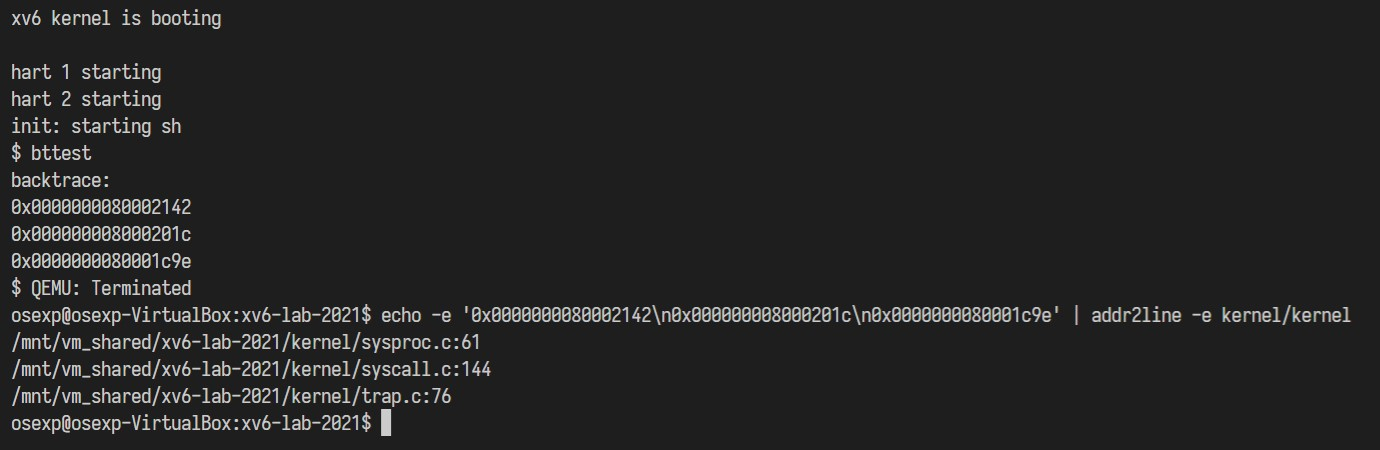
\includegraphics[width=0.8\textwidth]{traps_bttest.jpg}
  \caption{ 验证 \lstinline{backtrace()} 正确性的结果 }
\end{figure}
可见与预期相同,说明实现正确。

\section{实现定时器系统调用}

为了让一个进程能够在消耗一定的 CPU 时间后被告知,我们需要实现 \lstinline{sigalarm(n, fn)} 系统调用。用户程序执行 \lstinline{sigalarm(n, fn)} 系统调用后,将会在其每消耗 n 个 tick 的 CPU 时间后被中断并且运行其给定的函数 fn 。这个系统调用对于不希望占用过多 CPU 时间,或希望进行周期性操作的程序来说是及其有用的。此外,实现 \lstinline{sigalarm(n, fn)} 系统调用有利于我们学会如何构建用户态的中断和中断处理程序,这样就可以使用类似的方法使用户态程序可以处理缺页等常见的异常。

如果我们的实现正确,则运行 \lstinline{usertests} 和 \lstinline{alarmtest} 均会通过。

正确实现 \lstinline{sigalarm(n, fn)} 系统调用面临以下几个问题:
\begin{enumerate}
    \item 如何保存每个进程的 \lstinline{sigalarm} 参数;
    \item 如何并更新每个已经消耗的 tick 数;
    \item 如何在已经消耗的 tick 数符合要求时使进程调用中断处理过程 fn ;
    \item 中断处理过程 fn 执行完毕后如何返回。
\end{enumerate}

在解决这些问题前,我们先照例在 \lstinline{user/user.h} 加入两个系统调用的入口,分别用于设置定时器和从定时器中断处理过程中返回:
\begin{lstlisting}[language=C]
    int sigalarm(int ticks, void (*handler)());
    int sigreturn(void);
\end{lstlisting}

首先解决第一个问题,联想到 Lab System calls 中 trace 的实现,我们需要在每个进程的控制块的数据结构中加入存储 \lstinline{sigalarm(n, fn)} 中参数的项,即在 \lstinline{kernel/proc.h} 的 \lstinline{struct proc}中加入如下的项:
\begin{lstlisting}[language=C]
    int alarminterval;           // sys_sigalarm() alarm interval in ticks
    int alarmticks;              // sys_sigalarm() alarm interval in ticks
    void (*alarmhandler)();      // sys_sigalarm() pointer to the alarm handler
    int sigreturned;
\end{lstlisting}

然后在 \lstinline{kernel/proc.c} 的 \lstinline{allocproc(void)} 中对这些变量进行初始化:
\begin{lstlisting}[language=C]
static struct proc*
allocproc(void)
{
......
  // Initialize alarmticks
  p->alarmticks = 0;
  p->alarminterval = 0;
  p->sigreturned = 1;
  return p;
}
\end{lstlisting}

初始化后,在调用 \lstinline{sigalarm(n, fn)} 系统调用时,执行的 \lstinline{kernel/sysproc.c} 中的 \lstinline{sys_sigalarm()} 需根据传入的参数设置 \lstinline{struct proc} 的对应项:
\begin{lstlisting}[language=C]
uint64
sys_sigalarm(void)
{
  int ticks;
  uint64 handler;
  struct proc *p = myproc();
  if(argint(0, &ticks) < 0 || argaddr(1, &handler) < 0)
    return -1;
  p->alarminterval = ticks;
  p->alarmhandler = (void (*)())handler;
  p->alarmticks = 0;
  return 0;
}
\end{lstlisting}

可以在 \lstinline{sys_sigalarm(void)} 加入打印语句用于 debug ,确认参数传入无误后可以着手解决第二个问题。

如何并更新每个已经消耗的 tick 数,我们需要修改定时器中断发生时的行为,为每个有 \lstinline{sigalarm} 的进程更新其已经消耗的 tick 数。打开 \lstinline{kernel/trap.c} ,在 \lstinline{usertrap()} 中的判断是否为定时器中断的 if 语句块中加入对应的实现:

\begin{lstlisting}[language=C]
......
  if(which_dev == 2)
  {
    p->alarmticks += 1;
......
\end{lstlisting}

然后顺手解决第三个问题,判断该进程已经使用的 tick 数是否已经足以触发 alarm :
\begin{lstlisting}[language=C]
......
if(which_dev == 2)
{
  p->alarmticks += 1;
  if ((p->alarmticks >= p->alarminterval) && (p->alarminterval > 0))
  {
    p->alarmticks = 0;
......
  }
  yield();
}
......
\end{lstlisting}

若 ticks 达到了预先设定的值,则将计数器清零,并使得用户进程跳至预设的处理过程 fn 处执行。首先我们需要在 \lstinline{struct proc} 增设 \lstinline{alarmtrapframe} 用于备份进程当前的上下文:
\begin{lstlisting}[language=C]
......
  int alarminterval;           // sys_sigalarm() alarm interval in ticks
  int alarmticks;              // sys_sigalarm() alarm interval in ticks
  void (*alarmhandler)();      // sys_sigalarm() pointer to the alarm handler
  struct trapframe alarmtrapframe; // for saving registers
  int sigreturned;
......
\end{lstlisting}

然后,在 \lstinline{usertrap()} 中备份当前的上下文,并将用户态的程序计数器设置到 fn 处,然后完成该定时器调用,返回到用户态:
\begin{lstlisting}[language=C]
......
if(which_dev == 2)
{
  p->alarmticks += 1;
  if ((p->alarmticks >= p->alarminterval) && (p->alarminterval > 0))
  {
    p->alarmticks = 0;
    if (p->sigreturned == 1)
    {
      p->alarmtrapframe = *(p->trapframe);
      p->trapframe->epc = (uint64)p->alarmhandler;
      p->sigreturned = 0;
      usertrapret();
    }
  }
  yield();
}
......
\end{lstlisting}

这样整个触发 \lstinline{sigalarm} 的过程便成功完成了。此时还剩最后一个问题没有解决:当传入的 fn 执行完毕后,如何返回到进程正常的执行过程中。由于之前我们保存了进程执行的上下文,故而在 fn 调用 \lstinline{sigreturn()} 时,我们需要在内核态对应的 \lstinline{sys_sigreturn()} 中将备份的上下文恢复,然后返回用户态,该实现依然放在 \lstinline{kernel/sysproc.c} 中:
\begin{lstlisting}[language=C]
......
uint64
sys_sigreturn(void)
{
  struct proc *p = myproc();
  p->sigreturned = 1;
  *(p->trapframe) = p->alarmtrapframe;
  usertrapret();
  return 0;
}
......
\end{lstlisting}

至此,整个 alarm 机制便实现完成了。编译并启动 xv6 后,在 shell 中运行 \lstinline{alarmtest} ,即可看到预期的输出,如下图所示:
\begin{figure}[H]
  \centering
  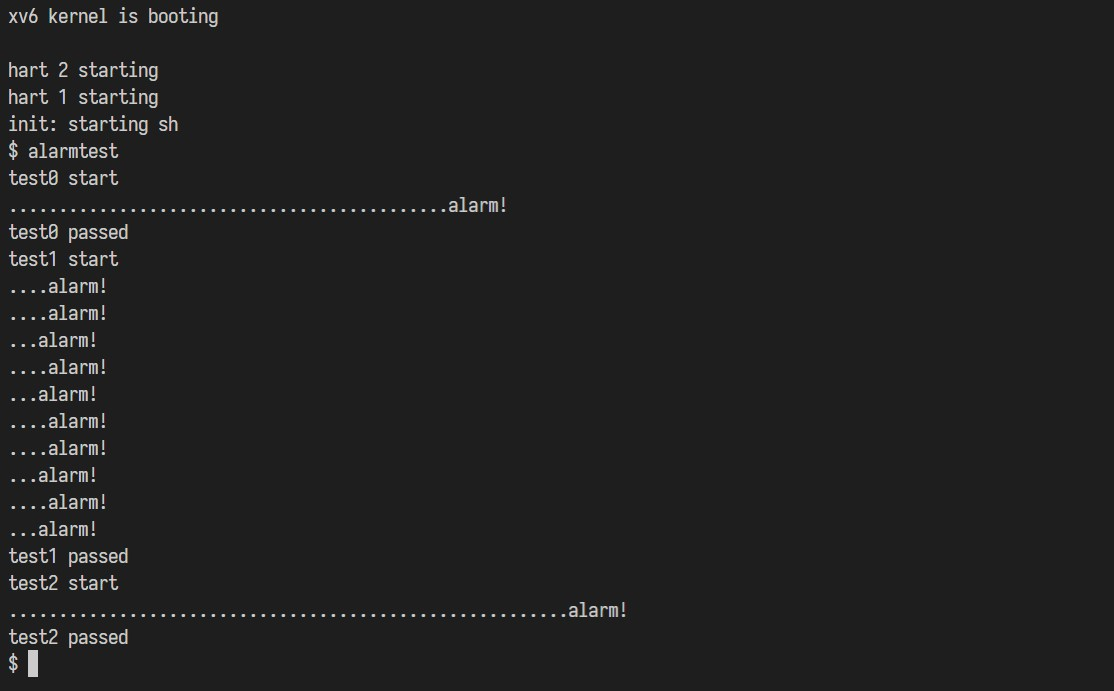
\includegraphics[width=0.8\textwidth]{traps_alarmtest.jpg}
  \caption{ 验证 alarm 机制的正确性 }
\end{figure}

\paragraph*{实验结果} 在完成 Lab Traps 中的所有实验后,根据 MIT 6.S081 的传统,需要在实验目录下创建一个名为 \lstinline{time.txt} 文本文件,其中只包含一行,为完成该实验的小时数。然后在终端中执行 \lstinline{make grade} ,即可对整个实验进行自动评分,笔者的结果如下:
\begin{figure}[H]
  \centering
  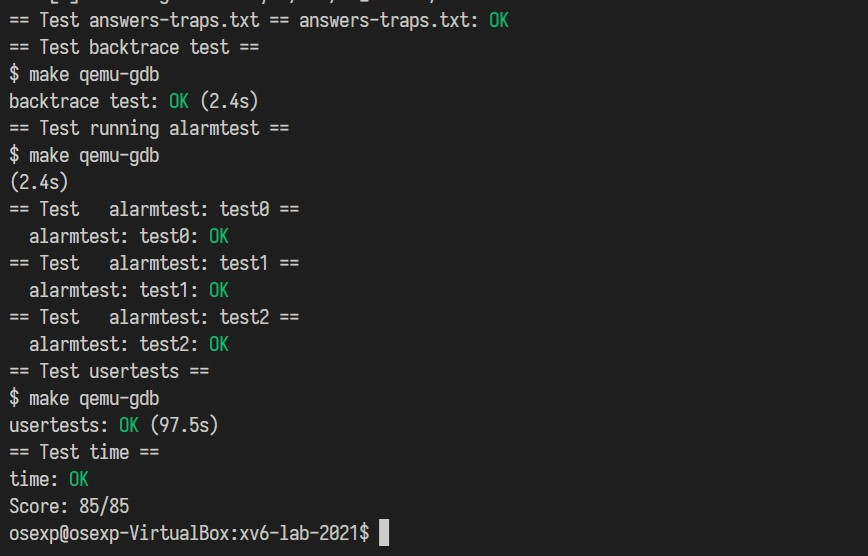
\includegraphics[width=0.8\textwidth]{traps_grade.jpg}
  \caption{ Lab Traps 的测评结果}
\end{figure}
可见测试全部通过,得分为满分。

\section{小结:RISC-V 的中断机制}

上面的实验中,我们首先了解了 RISC-V 的汇编及其 ABI 的一些内容,从而结合定时器中断来实现 alarm 的机制。实验中没有详细地讲解整个 RISC-V 的中断机制,故而笔者在这里对 xv6 涉及到的 RISC-V 的中断机制进行一个小结,这里我们主要参考 RISC-V 的手册 \textit{The RISC-V Instruction Set Manual: Volume II: Privileged Architecture} \footnote{\url{https://riscv.org/wp-content/uploads/2017/05/riscv-privileged-v1.10.pdf}} 。

我们首先考察 xv6 在启动时执行的一些初始化代码,在 \lstinline{kernel/start.c} 中,有如下的代码段:
\begin{lstlisting}[language=C]
......
  // set the machine-mode trap handler.
  w_mtvec((uint64)timervec);

  // enable machine-mode interrupts.
  w_mstatus(r_mstatus() | MSTATUS_MIE);
......
\end{lstlisting}

在 \lstinline{kernel/main.c} 中,有如下的代码段:
\begin{lstlisting}[language=C]
......
    trapinit();      // trap vectors
    trapinithart();  // install kernel trap vector
    plicinit();      // set up interrupt controller
    plicinithart();  // ask PLIC for device interrupts
......
\end{lstlisting}


这些初始化用的函数与中断相关。从这些初始化代码中不难发现, RiSC-V 管理中断的方式主要有几类:(裸机启动时的)定时器中断、来自内核的中断和通过 PLIC 管理的设备中断。

以来自内核态的中断为例展开介绍。对于内核态的中断,我们初始化时已经将对应的中断处理程序 \lstinline{kernel/kernelvec.S} 的地址放在了 STVEC 寄存器( Supervisor Trap Vector Base Address Register )中,见 \lstinline{kernel/trap.c} :
\begin{lstlisting}[language=C]
// set up to take exceptions and traps while in the kernel.
void
trapinithart(void)
{
  w_stvec((uint64)kernelvec);
}
\end{lstlisting}

这样,当内核态的中断发生时, CPU 会自动从 STVEC 寄存器指向的指令开始执行,即执行 \lstinline{kernel/kernelvec.S} 中的代码,具体工作为在内核栈中保存上下文,并调用 \lstinline{kernel/trap.c} 中的 \lstinline{kerneltrap()} ,调用完成后恢复栈中保存的上下文,继续运行内核原来正在进行的代码。

在 \lstinline{kerneltrap()} 中,涉及到一些描述中断状态的寄存器,其中较为重要的有 SEPC (  Supervisor Exception Program Counter 用于记录中断时的 PC )、 SSTATUS ( Supervisor Status Register 用于记录中断时的状态 )和 SCAUSE ( Supervisor Cause Register 用于记录中断的原因 )。 \lstinline{kerneltrap()} 会检查这些寄存器,从而判断中断是否合法。

类似的,对于由 \lstinline{ecall} 导致的中断,CPU 同样会自动从 STVEC 寄存器指向的指令开始执行,只是此时由于进程运行在用户态,故而 STVEC 寄存器在之前就已经被设为了 \lstinline{trampoline} 过程对应的首地址(在 \lstinline{kernel/trap.c} 中):
\begin{lstlisting}[language=C]
void
usertrapret(void)
{
......
  // send syscalls, interrupts, and exceptions to trampoline.S
  w_stvec(TRAMPOLINE + (uservec - trampoline));
......
\end{lstlisting}

在 \lstinline{kernel/trampoline.S} 调用 \lstinline{usertrap()} 后,处理器已经进入内核态(S态),此时 STVEC 寄存器的指向的地址又被设为了 \lstinline{kernel/kernelvec.S} 的地址:
\begin{lstlisting}[language=C]
void
usertrap(void)
{
......
  // send interrupts and exceptions to kerneltrap(),
  // since we're now in the kernel.
  w_stvec((uint64)kernelvec);
......
\end{lstlisting}

如此,通过 STVEC 寄存器的变化,我们可以根据需要方便地选取我们需要的中断处理程序 ( kernelvec 或 trampoline ),并且结合 SSTATUS 和 SCAUSE 寄存器的信息判断中断的种类,从而实现丰富的功能。

具体的一些例子,例如处理缺页异常的中断等,在下文的实验中将有所涉及。而对于 SSTATUS 和 SCAUSE 寄存器的各种取值及其含义,在手册 \textit{The RISC-V Instruction Set Manual: Volume II: Privileged Architecture} 中有详细的描述,需要时可以方便地查阅到。
